\documentclass[10pt, a4paper]{article}
\usepackage[slovene]{babel}
\usepackage[utf8]{inputenc}
\usepackage{lmodern}
\usepackage[T1]{fontenc}
\usepackage{eurosym}
\usepackage{amssymb}
\usepackage{amsfonts}
\usepackage{amsmath}
\usepackage{graphicx}
\usepackage{amsthm}

\begin{document}


\begin{titlepage}
\begin{center}
\vspace*{1cm}

\Large
Finančni praktikum - poročilo

\vspace{0.5cm}
\LARGE
\textbf{Tabu search on TSP}

\vspace{1.5cm}
\Large
Andraž Mur \\
Max Filip Uršič

\vspace{3cm}

\includegraphics[scale=1]{logo}


\vfill

\large Ljubljana, januar 2019

\end{center}
\end{titlepage}



\tableofcontents

\newpage



\section{Opis problema}

Najina naloga je bila implementacija metode isaknja Tabu Search na problemu potujočega trgovca. Tega sva se lotila z zapisom programa oziroma funkcije, ki s pomočjo omenjene metode v danem grafu poišče čim bolj optimalno pot. Nato sva morala program tudi uporabiti na več primerih, ki sva jih poiskala na medmrežju. Končne rešitve sva nato še primerjala z optimalnimi rešitvami danih problemov in iz rezultatov potegnila sklep o uspešnosti najinega programa.

\bigskip
\textbf{Problem potujočega trgovca} oz. \textbf{travelling salesman problem (TSP)} je NP-težak problem, ki govori o iskanju najkrajše poti med danim seznamom mest in vrnitvijo nazaj na začetek glede na dane razdalje med mesti. Gre za v praksi zelo uporabem problem, ki se uporablja na raznih področjih, kot so logistika, planiranje ter proizvodnja mikročipov, malo modificiran problem pa se uporablja tudi v astronomiji, kjer astronomi z njegovo pomočjo želijo čim bolj optimalno premikati teleskope in v sekvencioniranju DNA, kjer »mesto« predstavlja različne dele DNA-ja in »razdalja« predstavlja podobnost med le-temi.

\bigskip
Metoda \textbf{tabu search} je metaheoristična iskalna metoda, ki se uporablja v matematični optimizaciji. Gre za izboljšavo lokalnih optimizacijskih metod, ki za razliko od slednjih nima problemov z obstankom v lokalnih optimumih, saj sprosti njihovo osnovno načelo delovanja. Na vsakem koraku namreč dovoljuje slabše korake, torej iskanje rešitev, ki so slabše od trenutno optimalne, če boljših rešitev v okolici ni mogoče najti. Poleg tega upošteva tudi prepovedi v iskanju, kar preprečuje vračanje v že prej obiskane rešitve.Implementacija tabu search-a uporablja tudi spominske strukture, ki opisujejo že obiskane rešitve ter neka začetna pravila. Potencialna rešitev, ki je bila v bližnji preteklosti že obiskana ali krši kakšno od začetnih pravil, je označena kot ''tabu rešitev'', zato je algoritem v prihodnosti ne upošteva več.

\bigskip
Natančnejše delovanje zgoraj opisane metode na problemu potujočega trgovca pa je zaradi lažjega razumevanja same kode programa obrazloženo pri obravnavi delovanja najinega programa.

\bigskip
\bigskip
\begin{figure}[!h]
\centering
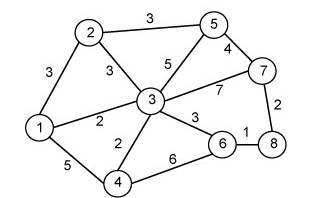
\includegraphics[scale=0.5]{slika1}
\caption{Primer problema potujočega trgovca}
\end{figure}




\section{Opis dela}

V tem razdelku si bomo podrobno ogledali zapisano kodo najinega programa. Za vsako zapisano funkcijo bova natančno utemeljila kaj počne, na kakšen način in zakaj.



\subsection{Zapis grafov v jeziku Python}

Na začetku sva se morala odločiti o tem, kako bova grafe sploh prevedla v programski jezik Python. Ker sva ugotovila, da so zelo pogosto grafi predstavljenimi s slovarji in ker se nama je to za najin program zdelo zelo priročno, sva se odločila za ta način.

\begin{verbatim}
vozlisca = [1, 2, 3, 4, 5, 6, 7, 8]
povezave = {1:[[2,3], [3,2], [4,5]],
            	2:[[1,3], [3,3], [5,3]],
            	3:[[1,2], [2,3], [4,2], [5,5], [6,3], [7,7]],
            	4:[[1,5], [3,2], [6,6]],
            	5:[[2,3], [3,5], [7,4]],
            	6:[[3,3], [4,3], [8,1]],
            	7:[[3,7], [5,4], [8,2]],
            	8:[[6,1], [7,2]]
           	}
\end{verbatim}

Zgornji zapis tako prikazuje vozlišča in povezave grafa iz slike 1, prevedene v želeno obliko.

\bigskip

Ker pa se grafi seveda pogosto zapisujejo tudi s pomočjo matrik sosednosti, sva se odločila za zapis dveh funkcij, ki prevedeta takšno matriko v slovar. Za zapis dveh različnih funkcij sva se odločila zato, ker so lahko grafi usmerjeni ali neusmerjeni, pri čemer velja, da je za neusmerjene grafe matrika sosednosti simetrična, zato prevajanje le-teh lahko precej poenostavimo.

\begin{verbatim}
def usmerjena_matrika_slovar(matrika):
    slovar = {}
    stevec1 = 1
    vozlisca = []
    for vrstica in matrika:
        sosedi = []
        stevec2 = 1
        for sosed in vrstica:
            if (sosed != 0) and (sosed != float('inf')):
                sosedi.append([stevec2, sosed])
            stevec2 += 1
        slovar[stevec1] = sosedi
        vozlisca.append(stevec1)
        stevec1 += 1
    return slovar, vozlisca
\end{verbatim}

Prva funkcija se uporablja za prevajanje matrike sosednosti usmerjenega grafa v slovar. Deluje na način, da za $i$-to vrstico matrike pregleda vse stolpce in v primeru, ko je vrednost elementa različna od 0 (vozlišče ni sam svoj sosed) in $\infty$ (vozlišči si nista sosedni) v seznam sosedov $i$-tega vozlišča doda $j$-to vozlišče, če se nahajamo v $j$-tem stolpcu matrike. To se seveda zgodi za vsak $i$, torej za vsako vrstico matrike sosednosti.

Na koncu se je sicer izkazalo, da so vsi najini primeri neusmerjeni grafi, vendar sva se vseeno odločila, da funkcijo obdrživa.

\begin{verbatim}
def neusmerjena_matrika_slovar(matrika):
    n = len(matrika)
    slovar = {}
    vozlisca = []
    for i in range(0, n):
        slovar[i] = []
        vozlisca.append(i)
    for i in range(0, n):
        for j in range(i, n):
            dolzina = matrika[i][j]
            if (dolzina != 0) and (dolzina != float('inf')):
                slovar[i].append([j, dolzina])
                slovar[j].append([i, dolzina])
    return slovar, vozlisca
\end{verbatim}

Funkcija za prevajanje matrike sosednosti neusmerjenega grafa deluje precej podobno prejšnji, razlikuje se le v tem, da si ogleduje le elemente matrike, ki ležijo nad diagonalo, saj so za takšne grafe, kot že omenjeno, matrike sosednosti simetrične.

\bigskip

Ob zaključku projekta, torej ob iskanju in reševanju praktičnih primerov, pa sva ugotovila tudi, da so praktični problemi pogosto predstavljeni s koordinatami mest, ki jih mora trgovec obiskati, povezave pa so možne med vsemi mesti, kar pomeni, da gre v resnici za polne grafe. Razdalja med posameznimi mesti se izračuna precej enostavno, in sicer kot najkrajša razdalja med lokacijima mest. Prav zaradi tega dejstva sva zapisala še funkcijo, ki iz dane datoteke s koordinatami sestavi matriko sosednosti za graf, s pomočjo katere z zgoraj opisanima funkcijama problem prevedemo v želeno obliko. Za pretvorbo direktno v slovar se nisva odločila, saj sva ugovotvila da je takšen način prevajanja časovno manj zahteven.

\bigskip
Spodaj predstavljena funkcija torej počne ravno slednje, s tem, da si na začetku iz vsake vrstice datoteke izpiše vrednosti, nato si definira matriko velikosti $n \times n$ z vrednostmi $\infty$, katere ob koncu še nadomesti z dejanskimi razdaljami med mesti.

\newpage

\begin{verbatim}
def prevedba_koordinat(datoteka):
    koordinate = []
    with open (datoteka) as file:
        for vrstica in file:
            koordinate.append(vrstica.split())
    n = len(koordinate)
    matrika_sosednosti = []
    for i in range(0, n-1):
        matrika_sosednosti.append((n-1)*[float('inf')])
    for i in range(0, n-1):
        for j in range(i, n-1):
            prvi_kraj = (float(koordinate[i][1]), float(koordinate[i][2]))
            drugi_kraj = (float(koordinate[j][1]), float(koordinate[j][2]))
            razdalja = ((drugi_kraj[0] - prvi_kraj[0])**2 
	                        + (drugi_kraj[1] - prvi_kraj[1])**2)**(1/2)
            matrika_sosednosti[i][j] = razdalja
            matrika_sosednosti[j][i] = razdalja
    return matrika_sosednosti
\end{verbatim}




\subsection{Osnovne funkcije}

Potem, ko sva se dokončno dogovorila o načinu zapisovanja grafov, sva lahko začela z definiranjem resnejših pomožnih funkcij, s pomočjo katerih bo na koncu deloval končen program. Funkcije seveda delujejo na grafih, ki so predstaljeni s slovarji na zgoraj opisan način.

\begin{verbatim}
def dolzina_poti(pot, povezave):
    dolzina = 0
    for i in range(0, len(pot)-1):
        vozlisce = pot[i]
        sosedi = []
        for sosed in povezave[vozlisce]:
            sosedi.append(sosed[0])
            if pot[i+1] == sosed[0]:
                dolzina += sosed[1]
        if pot[i+1] not in sosedi:
            return float('inf')
    return dolzina
\end{verbatim}

Prva pomožna funkcija se, tako kot to povesta že njeno ime in opis, uporablja za izračun dolžine dane poti glede na dan slovar povezav. Na začetku dolžino poti postavimo na 0 in se začnemo gibati po poti. Nato za vsako voszlišče, ki ga dosežemo sestavimo seznam sosedov in si ogledamo, če naslednje vozlišče v poti leži v njem. Če to drži, dolžini dodamo razdaljo med tema dvema vozliščema in postopek nadaljujemo, v nasprotnem primeru pa pot sploh ne obstaja, zato funkcija za dolžino poti vrne $\infty$.

\newpage

\begin{verbatim}
def okolica_poti(vozlisca, pot, povezave):
    n = len(pot)
    okolica = []
    sosedi = {}
    for i in vozlisca:
        sosedi[i] = []
        for sosed in povezave[i]:
            sosedi[i].append(sosed[0])
    for i in range(0, n-3):
        for j in range(i+3, n):
            if (pot[i] in sosedi[pot[j-1]]) and (pot[i+1] in sosedi[pot[j]]):
                nova_pot = pot[:]
                nova_pot[i+1:j] = nova_pot[i+1:j][::-1]
                if nova_pot != pot:
                    okolica.append(nova_pot)
    return okolica
\end{verbatim}

Naslednjo sva definirala funkcijo za iskanje okoliških poti glede na dano pot. Funkcija najprej ustvari prazen seznam sosedov, kamor bo nato vpisovala vse sosede. Sosedi v primeru TSP so tiste poti, ki jih iz dane dobimo z zamenjavo dveh vozlišč v poti, zaradi česar moramo posledično zamenjati še vrstni red vseh vozlišč med zamenjanima dvema. Če imamo na primer zaporedje vozlišč $v_1, \dots , v_i, v_{i+1}, \dots , v_{j-1}, v_j, \dots, v_n$ ter sta vozlišči $v_i$ in $v_{j-1}$ sosednji, t.j. v grafu med njima obstaja povezava, enako pa velja za vozlišči $v_j$ ter $v_{i+1}$, je potem pot $v_1, \dots , v_i, v_{j-1}, v_{j-2}, \dots ,v_{i+2}, v_{i+1}, v_j, \dots, v_n$ sosednja.  

Funkcija nato ustvari nov slovar sosedov brez zapisanih razdalj med vozlišči, saj nas le-te ne zanimajo. Nato pa se z dvema zankama spustimo čez vsa vozlišča ter preverjamo, če je zgoraj omenjen pogoj izpolnjen. V primeru ko to res drži, elemente nove poti premečemo na opisan način in jo dodamo v seznam \texttt{okolica}.




\subsection{Iskanje začetne rešitve}

Na nekaj več težav pa sva naletela pri zapisu funkcije, ki v danem grafu poišče začetno rešitev. Ločiti sva namreč morala primere, ko se do tedaj zapisana pot ni bila zmožna nadaljevati in se je zato morala vrniti eno ali več vozlišč nazaj. Ta problem sva rešila s pomočjo števca, ki meri način prihoda v neko vozlišče, t.j. ki nam pove, če smo do vozlišča prišli z običajnim korakom naprej (v tem primeru ima števec vrednost 0) ali pa če smo do njega prišli s korakom nazaj (taktrat ima števec vrednost 1).

\newpage

\begin{verbatim}
def poisci_resitev(vozlisca, povezave):
    zacetek = vozlisca[0]
    pot = [zacetek]
    vozlisce = zacetek
    naslednji_koraki = []
    stevec = 0
    while True:
        if stevec == 0:
            sosedi = []
            for sosed in povezave[vozlisce]:
                if sosed[0] not in pot:
                    sosedi.append(sosed[0])
            naslednji_koraki.append(sosedi)
        izbire = naslednji_koraki[-1][:]
        if izbire == []:
            pot.remove(vozlisce)
            naslednji_koraki.remove(izbire)
            naslednji_koraki[-1].remove(vozlisce)
            vozlisce = pot[-1]
            stevec = 1
        else:
            random.shuffle(izbire)
            novo_vozlisce = izbire.pop(0)
            pot.append(novo_vozlisce)
            if len(pot) == len(vozlisca):
                koncni_sosedi = []
                for sosed in povezave[novo_vozlisce]:
                    koncni_sosedi.append(sosed[0])
                if zacetek in koncni_sosedi:
                    pot.append(zacetek)
                    return pot
                else:
                    pot.remove(novo_vozlisce)
                    naslednji_koraki[-1].remove(novo_vozlisce)
                    vozlisce = pot[-1]
                    stevec = 1
            else:
                vozlisce = novo_vozlisce
                stevec = 0
\end{verbatim}

Ta funkcija na začetku razbere prvo vozlišče in si ga shrani v spremenljivko \texttt{zacetek}. To stori zato, ker sva se odločila, da se bo vsaka pot znotraj iskanja začela v prvem vozlišču in se tam seveda tudi končala. Za to sva se odločila, ker so vse poti sklenjene in je posledično povsem irelevantno v katerem vozlišču se začne, prvo vozlišče pa sva za ta namen izbrala zaradi boljše preglednosti. Poleg tega \texttt{zacetek} dodamo tudi v pot, ga izberemo za prvotno vozlišče in nato zapišemo \texttt{while True} zanko, ki deluje dokler ne najdemo ustrezne poti.

Na vsakem koraku si za vozlišče, v katerem se trenutno nahajamo, ogledamo njegove sosede, ki še niso bili obiskani ter jih zapišemo v seznam \texttt{sosedi}. Ta seznam nato dodamo v seznam naslednjih korakov, ki je na začetku seveda prazen. Zadnji element tega seznama nam pove, v katera vozlišča se lahko premaknemo v naslednjem koraku. Če je torej le-ta prazen, poti ne moremo nadaljevati, zato moramo storiti korak nazaj, trenutno vozlišče izbrisati iz poti, prav tako pa ga moramo odstaniti tudi iz zadnjega elementa seznama \texttt{naslednji\_koraki}, saj očitno ob izbiri tega vozlišča poti ne moremo sestaviti.

V nasprotnem primeru pa iz seznama možnih kandidatov najprej naključno izberemo eno vozlišče in ga dodamo v pot. Za tem si ogledamo, če je dolžina poti že enaka številu vozlišč, saj smo v tem primeru že obiskali vsa vozlišča, tako da je potrebna le še vrnitev nazaj v izhodiščno vozlišče. V primeru, ko obstaja povezava med zadnjim vozliščem v poti in začetkom, v pot dodamo \texttt{zacetek} in vrnemo pot. V naprotnem primeru pa torej poti ne moremo dokončati, zaradi česar moramo, podobno kot je opisano zgoraj, narediti en korak nazaj, s čimer smo ugotovili, da ta kandidat ni primeren za nadaljevanje poti. V primeru, ko vseh vozlišč še nismo obiskali, pa za naslednje vozlišče določimo izbranega kandidata ter naredimo standarden korak naprej.




\subsection{Končni program}

S pomočjo vseh zgoraj opisanih pomožnh funkcij in psevdokode za Tabu Search na problemu potujočega trgovca sva na koncu še zapisala funkcijo \texttt{tabu\_search}, ki za dan graf s pomočjo te metode poišče čim boljšo rešitev.

\begin{verbatim}
Input: TabuList_size
Output: S_best

S_best <- ConstructInitialSolution()
TabuList <- emptyset()
While (not StopCondition())
    CandidateList <- emptyset()
    For (S_candidate in S_best_neighborhood)
        If (not ContainsAnyFeatures(S_candidate, TabuList))
            CandidateList <- S_candidate
        End
    End
    S_candidate <- LocateBestCandidate(CandidateList)
    If (Cost(S_candidate) < Cost(S_best))
        S_best <- S_candidate
        TabuList <- FeatureDifferences(S_candidate, S_best)
        While (TabuList > TabuList_size)
            DeleteFeature(TabuList)
        End
    End
End
Return (S_best)
\end{verbatim}

Iz zgornje psevdokode lahko hitro razumemo delovanje metode Tabu Search in posledično deovanje najinega programa oz. funkcije za reševanje problema potujočega trgovca. Na začetku si kot najboljšo pot shranimo neko naključno poiskano rešitev, za tabu seznam pa definiramo nov prazen seznam. Nato pa postopek izboljšave ponavljamo doker ni izpolnjen zaustavitven kriterij, kar v najinem primeru predstavlja dovoljšnje število korakov. 

Postopek izboljšave poteka tako, da najprej poiščemo okolico trenutnega optimuma, pri čemer izločimo tiste elemente, ki so že vsebovani v tabu seznamu, torej smo jih že obiskali ne dolgo tega. Nato iz dobljene okolice poiščemo tisto rešitev, ki ima od vseh kandidatov najboljšo vrednost ter jo primerjamo s trenutnim optimumom. Če je vrednost rešitve boljša, torej za najin primer če je izbrana pot krajša od do tedaj optimalne, potem za optimum vzamemo to rešitev ter jo dodamo v tabu seznam. V primeru, da je po tem dolžina tabu seznama večja od omejitve, prvi element le-tega odstranimo ter postopek na enak način nadaljujemo, dokler, kot že omenjeno, ni dosežen zaustavitven pogoj.

Najina funkcija sprejme še 3 dodatne parametre, in sicer \texttt{max\_koraki}, s katerim določimo število korakov funkcije, \texttt{max\_tabu}, ki določa maksimalno dolžino tabu seznama ter \texttt{izpis}, s katerim določimo na koliko korakov naj nam funkcija izpiše dolžino trenutno optimalne poti, kar koristi pri lažji predstavi delovanja funkcije glede na število korakov.





\section{Eksperimentiranje}

Funkcijo \texttt{tabu\_search} sva nato uporabila na več testnih primerih, ki so se med seboj razlikovali predvsem v dolžini grafov, oziroma načinu, kako so le-ti predstavljeni. Najin osnovni primer, t.j. primer iz slike 1, sva izbrala predvsem zaradi preprostosti, saj sva ga lahko reševala tudi sama brez pomoči računalnika ter posledično na njem testirala pravilno delovanje vseh definiranih funkcij. Za tem pa sva se lotila reševanje bolj resnih oz. večjih problemov, kjer sva imela opravke s planarnimi grafi, ki večinoma predstavljajo države, mesta ali pokrajine. Na teh sva iskala najkrajše poti med lokacijami (vozlišči), ob predpostavki, da morava obiskati vse in se nato vrniti v začetno točko. Pri planarnih grafih je potrebno omeniti tudi, da so le-ti vedno polni, kar pomeni, da lahko iz kateregakoli mesta odidemo v katerokoli drugo.

Vsi primeri, predstavljeni v nadaljevanju, razen prvega so sicer dostopni na povezavah, navedenih pod literaturo.



\subsection{Osnovni primer}

Kot je že omenjeno je bila glavna naloga tega primera, da sva lahko na njem testirala funckije, ki sva jih definirala. \texttt{tabu\_search} hitro vrne optimalno rešitev in pot, saj je graf res precej manjhen. Posledično že z določitvijo parametra $\texttt{max\_tabu} = 0$ dosežemo, da tabu seznam po nekaj korakih že vsebuje vse možnosti, zaradi česar se funkcija predčasno zaključi. Optimalnih poti pa je sicer več možnih, ena od teh je npr. $1, 3, 4, 6, 8, 7, 5, 2, 1$ z dolžino 23.

\begin{center}
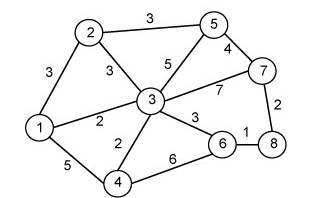
\includegraphics[scale=0.4]{slika1}
\end{center}



\subsection{Primer Bavarska velikosti 29}

Prvi večji testni primer, ki sva ga izvedla, je bil za pokrajino Bavarsko, pri katerem so bile podane koordinate 29 mest. Pri tem primeru nama je pri dobri izbiri parametrov \texttt{max\_koraki} ter \texttt{max\_tabu} funkcija vrnila zelo dober približek poti že po prvem zagonu. Le-ta se je ponavadi še izboljšal, ko sva program pognala do trikrat, več ponovitev pa je bilo že trivialno izvajat, saj so bili dobljeni rezultati že enaki prejšnjim. 

Funkcija je pri problemu bavarska najbolje delovala, če smo vrednost parametra \texttt{max\_tabu} izbrali nekje med 50 in 60. V primeru, ko je bil ta izbran precej nižje (okoli 25), se je funkcija prevečkrat vrnila v slabe poti in se posledično ni uspela izboljšati. Po drugi strani pa je bilo ob preveliki vrednosti parametra (okoli 100) preveč poti prepovedanih in prostora za izboljšavo posledično prav tako ni bilo. Parameter \texttt{max\_koraki} pa je bilo v veliki večini primerov brezpredmetno povečevati na več kot 150, saj so bile vrednosti, ki jih je funkcija vračala od 75 koraka naprej enake.



\subsection{Primer Eilon velikosti 51}

Drugi testni primer na planarnih grafih je bil za Eilon, kjer je bilo število mest že večje (51). Pri tem problemu sva po večih zagonih pri različnih postavitvah parametrov vedno prišla do zelo podobnih rešitev, ki se med parametri niso zelo razlikovale. Rešitev se je še najboljše približala optimalni (426), ko sva za parameter \texttt{max\_tabu} vzela vrednost 50 in je takrat znašala 436. Pri ostalih izbirah (25 in 100) pa je funkcija po nekaj zagonih vedno našla rešitev, ki se je gibala v okolici 440. Zaradi enakega razloga kot pri problemu Bavarske je bilo brezpredmetno povečevati število korakov na več kot 150, saj se je rešitev ponavadi ustalila pri 100 korakih.



\subsection{Primer Eilon velikosti 101}

Tretji testni primer na planarnih grafih je bil prav tako za Eilon, le da je bilo tokrat 101 vozlišč, kar se je znantno poznalo pri času, ki ga je program potreboval za reševanje problema. Tudi tu sva dobila različno dobre približke v odvisnosti od parametrov,  predvsem od parametra \texttt{max\_tabu}. Vpliv slednjega na delovanje funkcije sva predstavila v spodnjem grafu. Program sva večkrat pognala in iz rešitev izbrala najboljše rezultate, ki jih je vrnil za različno vrednost parametra \texttt{max\_tabu}. Ker je bil graf tu večji, je bila najboljša izbira parametra (kot sva pričakovala) 100, medtem ko pa se pri 25 in 50 gibanje rešitev ni zelo razlikovalo. Drugi parameter \texttt{max\_koraki}, pa je zaradi enakih razlogov kot prej brezpredmetno povečevati na več kot 200, kar je prav tako razvidno iz grafa.

\begin{center}
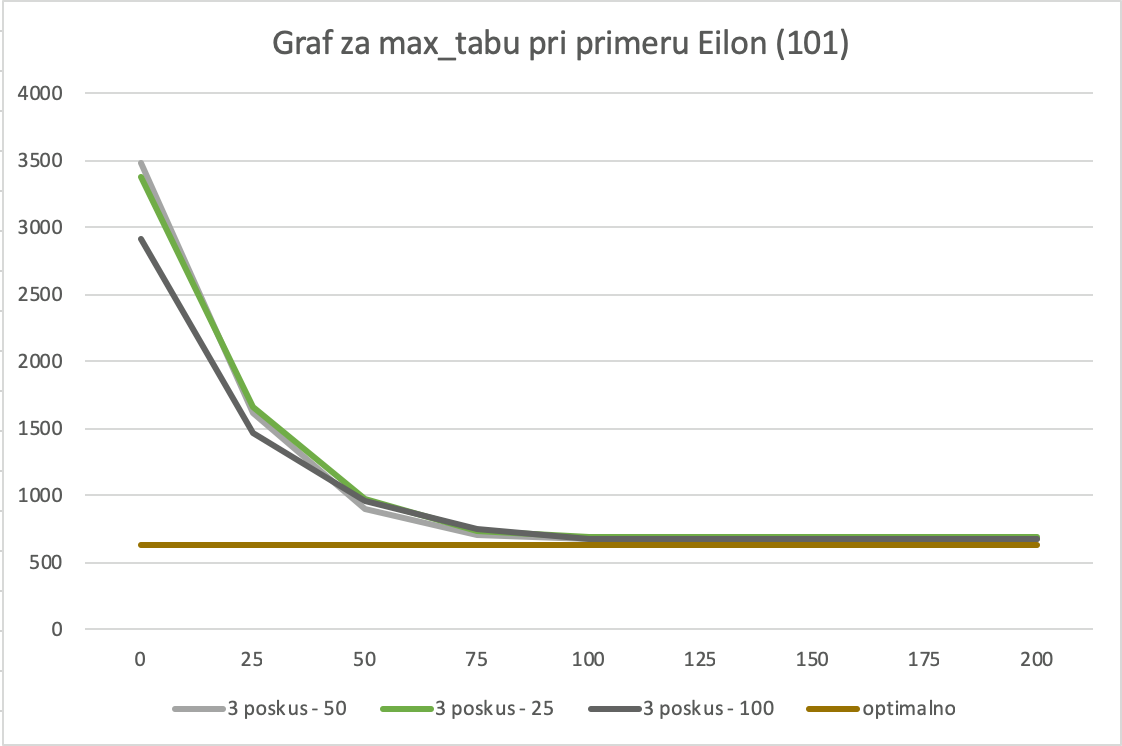
\includegraphics[scale=0.3]{graf}
\end{center}




\section{Zaključek}

Med programiranjem funkcij sva dobro obnovila znanje programiranja v jeziku Python ter podrobno spoznala metodo Tabu Search na problemu potujočega trgovca. S programom sva imela kar nekaj težav, predvsem z pomožnima funkcijama \texttt{okolica\_poti} ter \texttt{poisci\_resitev}, saj sva si na začetku narobe predstavljala, kaj v najinem primeru predstavlja soseda. Ko nama je uspelo razrešiti vse nejasnosti, sva problem uspešno testirala na več primerih, kjer sva ugotovila, da je v najinem končnem programu \texttt{tabu\_search} najpomembnejši parameter \texttt{max\_tabu}, katerega optimalna vrednost pa se razlikuje od primera do primera, glede na število vozlišč, ki jih testiran graf ima.





\begin{thebibliography}{4}
\bibitem{prvi}
MP-TESTDATA - The TSPLIB Symmetric Traveling Salesman Problem Instances (online), 5. 1. 2019. Dostopno na:
\\\texttt{http://elib.zib.de/pub/mp-testdata/tsp/tsplib/tsp}

\bibitem{TSP}
National Traveling Salesman Problems (online), 5. 1. 2019. Dostopno na:
\\\texttt{http://www.math.uwaterloo.ca/tsp/world/countries.html}

\bibitem{tabu}
Tabu Search (online), 5. 1. 2019. Dostopno na:
\\\texttt{https://en.wikipedia.org/wiki/Tabu\_search}

\bibitem{clever}
Tabu Search (online), 5. 1. 2019. Dostopno na:
\\\texttt{http://www.cleveralgorithms.com/nature-inspired/stochastic/tabu\_search.html}
\end{thebibliography}























\end{document}